\documentclass[12pt]{article}
\usepackage[margin=1in]{geometry} 
\usepackage{amsmath,amsthm,amssymb,amsfonts}
\usepackage{enumitem} 
\usepackage{graphicx}
\graphicspath{ {../P2/} }
\usepackage{listings}
\usepackage{color}
 
\definecolor{codegreen}{rgb}{0,0.6,0}
\definecolor{codegray}{rgb}{0.5,0.5,0.5}
\definecolor{codepurple}{rgb}{0.58,0,0.82}
\definecolor{backcolour}{rgb}{0.95,0.95,0.92}
 
\lstdefinestyle{mystyle}{
    backgroundcolor=\color{backcolour},   
    commentstyle=\color{codegreen},
    keywordstyle=\color{magenta},
    numberstyle=\tiny\color{codegray},
    stringstyle=\color{codepurple},
    basicstyle=\footnotesize,
    breakatwhitespace=false,         
    breaklines=true,                 
    captionpos=b,                    
    keepspaces=true,                 
    %numbers=left,                    
    numbersep=5pt,                  
    showspaces=false,                
    showstringspaces=false,
    showtabs=false,                  
    tabsize=2
}
 
\lstset{style=mystyle}
 
\newcommand{\N}{\mathbb{N}}
\newcommand{\Z}{\mathbb{Z}}
\newcommand{\C}{\mathcal{C}}
\newcommand{\D}{\mathcal{D}}
 
\begin{document}
 
\title{Numerical methods for linear regression}
\author{[redacted]}
\maketitle
 
In this paper we explore methods for regression of simple linear models. In section 1, we begin by discussing a popular method for the numerical optimization of differentiable cost functions: gradient descent. We compare two variants of its implementation, batch gradient descent (BGD) and stochastic gradient descent (SGD), and discuss their convergence characteristics. In section 2, we benchmark the performance of gradient descent on the least squares fitting of simple linear models on generated data and compare its performance against the analytic solution. Since the generated data is known The simplicity of the data allows us to study the effect of model selection as we consider both polynomial basis functions and cosine basis functions for the fitted model. Finally, in sections 3 and 4, we explore the effect of L2- and L1-norm regularization, respectively, in model optimization and discuss their implications on the bias-variance tradeoff of the fitted parameters.

\section{Gradient Descent}

\section{Linear Basis Function Regression}

Linear models are a popular choice of regression model due to their computational simplicity and interpretability. In a linear model, the model $f$ used to predict the observed data is expressed as a linear combination of terms:
$$ f(w,x) = \sum_i w_ig_i(x) $$
where $g$ are basis functions that transform the input data $x$, and $w$ are weights on each term. Note that while $g$ may involve a nonlinear transformation of $x$; the model is considered a linear model as long as it is linear in the parameters $w$. We can express $f$ in matrix form as
$$f(w,x) = \Phi w$$
where the ith column vector of $\Phi$ is $g_i(x)$. 

In the fitting of $n$ pairs of $(x,y)$ observational data, we first choose the functional form via selection of the basis functions $g_i$, and subsequently fit our model parameters $w_i$ by minimizing the sum of the square error (SSE) between the model prediction and the observed output: 
$$ argmin_w \theta(w) = argmin_w \sum_n (y_n - f(w,x_n))^2$$ % todo: define indexing variables
Alternative formulations of the problem exist where we simultaneously consider the space of potential models in the fitting process, however, that is outside the scope of this work.

The minimization of $\theta$ for linear basis functions has a closed form solution (Equation [below]). In the subsequent sections, we explore the tradeoffs between different choices of basis functions, and we use the analytically computed weights for various choices of linear basis function to benchmark gradient descent minimization of $\theta$ and gain intuition on its convergence properties. 

$$w = (\Phi^T\Phi)^{-1}\Phi^Ty$$
% todo: Talk about connection to maximum likelihood?
% todo: look up how to number equations...



\subsection{Linear regression with a polynomial basis}

Eleven data points were generated under the following function with added noise:
$$ f(x) = cos(\pi x) + 1.5cos(2\pi x); x \in [0,1]$$ 

Ignoring the true basis, we instead try to fit the data using a polynomial basis $\phi_0(x) = 1, \phi_1(x) = x, \phi_2(x) = x^2, ... , \phi_M(x) = x^M$, with GLS.  Figure 1 shows the tradeoff between model complexity and the quality of fit to the *training data*. At M=0 and M=1, the model is too simple and we have a large SSE. At the other extreme, with M=10, the model is able to exactly fit in the input data (SSE=0), however, with this little data, we are extremely susceptible to overfitting to the noise in the input data. Indeed, at high values of M, our fitted polynomials oscillate between points, thus deviating from the true model even within the range of the training data. Furthermore, since we know the true model is a sum of cosines, the extrapolative power of any of these polynomial basis models outside the training range of $x \in [0,1]$ is poor, thus underscoring the danger of using a model to make predictions outside the range of its training data.

\begin{figure}
\caption{As the polynomial order M increases, the sum of square error (SSE) between the fitted polynomial and the input data decreases, however the risk of overfitting increases.}
\begin{center}
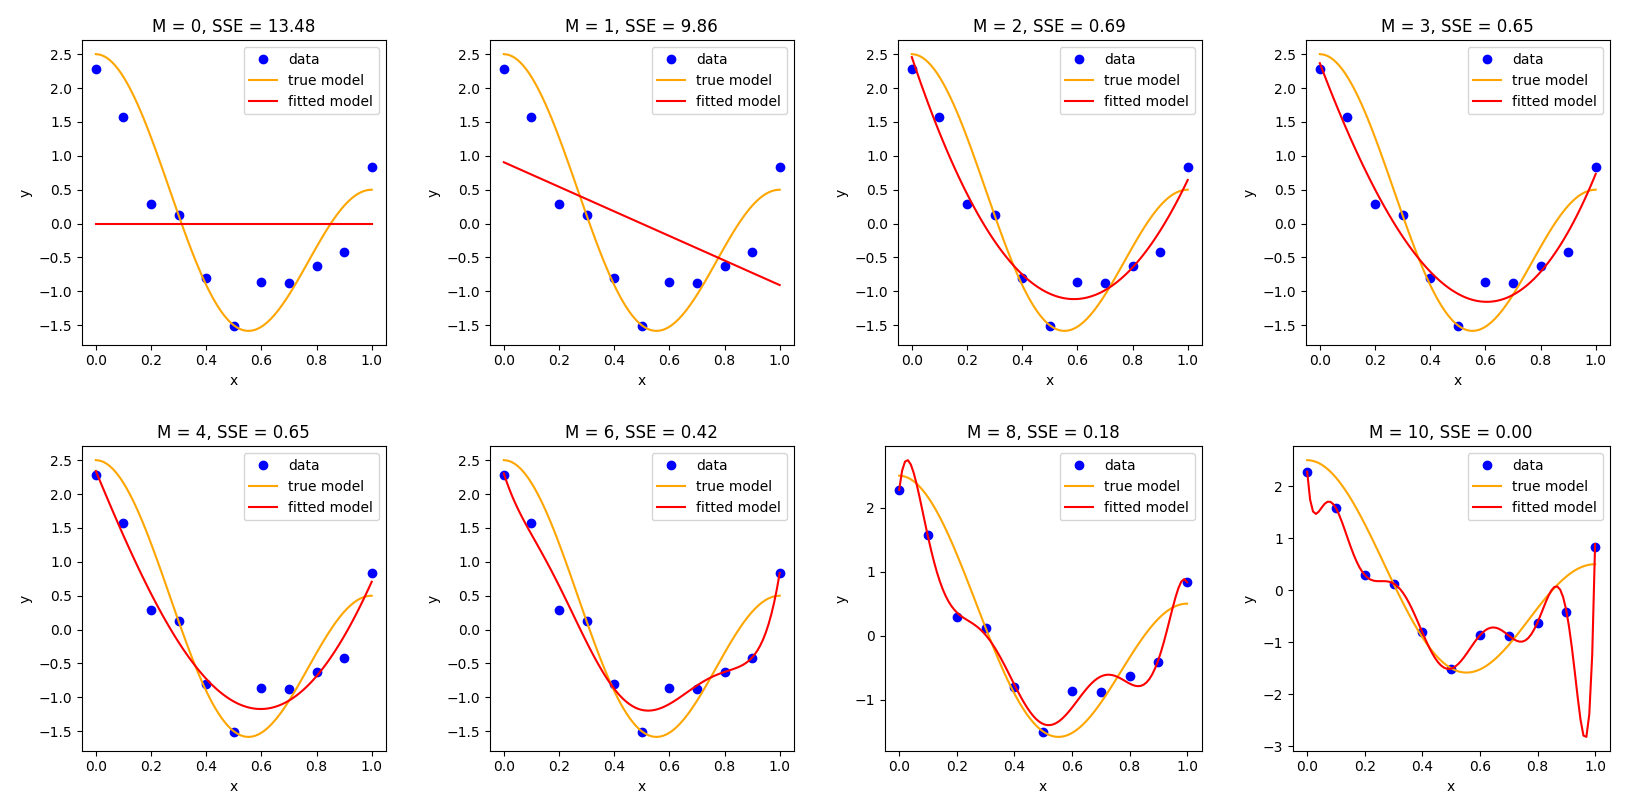
\includegraphics[width=450px]{all_regress_m}
\end{center}
\end{figure}

\subsection{Performance of BGD and SGD}

Next we explore the performance of BGD and SGD at reproducing the optimized weights for linear polynomial basis functions. 

\subsection{Linear regression with a cosine basis}

Using a cosine basis of the form $\phi_1(x) = cos(\pi x), \phi_2(x) = cos(2\pi x), ... , phi_M(x) = cos(M\pi x)$, we fit the same data as in Section 2.1 (Figure 2).

\begin{figure}
\caption{As the cosine order M increases, the sum of square error (SSE) between the fitted model and the input data decreases, however the risk of overfitting increases.}
\begin{center}
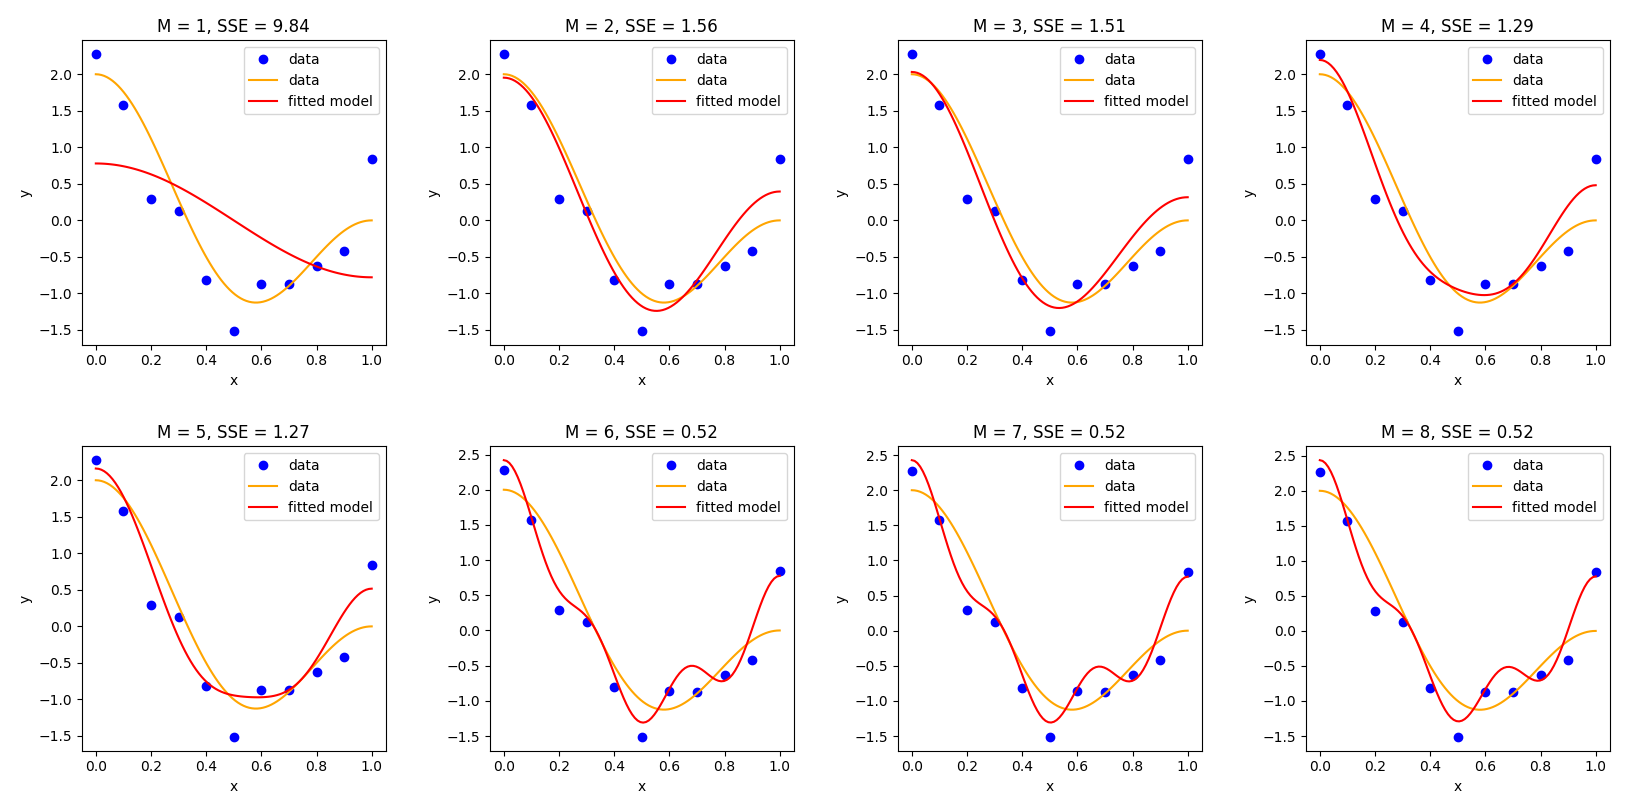
\includegraphics[width=450px]{all_regress_cos}
\end{center}
\end{figure}


\section{Ridge Regression}

\section{Sparsity and LASSO}

\section{Conclusions}

\section{References}

 \end{document}